%%%%%%%%%%%%%%%%%%%%%%%%%%%%%%%%%%%%%%%%%%%%%%%%%%%%%%%%%%%%%%%%%%%%%%%%%%%%%%%%%
%%%%%                             SETTINGS                                   %%%%
%%%%%%%%%%%%%%%%%%%%%%%%%%%%%%%%%%%%%%%%%%%%%%%%%%%%%%%%%%%%%%%%%%%%%%%%%%%%%%%%%
\documentclass{article}

\usepackage{inputenc}
\usepackage{csquotes}
\usepackage[a4paper, total={6in, 9.2in}]{geometry}
\usepackage{hyperref}
\usepackage{dsfont}
\usepackage{amsmath,amssymb,dsfont}
\usepackage{graphicx}
\usepackage{indentfirst}
\usepackage{caption}
\usepackage{subcaption}
\usepackage{booktabs}
\usepackage{setspace}
\usepackage{indentfirst}
\usepackage[inline]{enumitem}
\usepackage{lscape}

\usepackage{tikz}
\usetikzlibrary{decorations.pathreplacing, positioning, arrows.meta}

\linespread{1.2}
\setlength{\parskip}{.5em}%

\usepackage[backend = bibtex,
		   style = authoryear,
		   maxnames = 5,
		   maxcitenames = 3,
		   doi = false,
		   eprint = false]{biblatex}
\addbibresource{biblio.bib}

\newcommand{\aref}[1]{\hyperref[#1]{Appendix~\ref{#1}}}

\def\equationautorefname~#1\null{%
  equation~(#1)\null
}

%%%%%%%%%%%%%%%%%%%%%%%%%%%%%%%%%%%%%%%%%%%%%%%%%%%%%%%%%%%%%%%%%%%%%%%%%%%%%%%%%
%%%%%                                TITLE                                   %%%%
%%%%%%%%%%%%%%%%%%%%%%%%%%%%%%%%%%%%%%%%%%%%%%%%%%%%%%%%%%%%%%%%%%%%%%%%%%%%%%%%%

\title{Do Minimum Wages Increase Rents? 
	   Evidence from U.S. Zipcodes using High Frequency Data \thanks{We thank ...}}
\author{Gabriele Borg \and Diego Gentile Passaro \and Santiago Hermo
		\footnote{Borg: Department of Economics, Brown University (email: 
		\url{gabriele_borg@brown.edu}); 
		Gentile Passaro: Department of Economics, Brown University (email: 
		\url{diego_gentile_passaro@brown.edu}); 
		Hermo: Department of Economics, Brown University (email: 
		\url{santiago_hermo@brown.edu}).}
		}
\date{\today}


%%%%%%%%%%%%%%%%%%%%%%%%%%%%%%%%%%%%%%%%%%%%%%%%%%%%%%%%%%%%%%%%%%%%%%%%%%%%%%%%%
%%%%                              STRUCTURE                                  %%%%
%%%%%%%%%%%%%%%%%%%%%%%%%%%%%%%%%%%%%%%%%%%%%%%%%%%%%%%%%%%%%%%%%%%%%%%%%%%%%%%%%

\begin{document}

\maketitle

\begin{abstract}
    \noindent In this paper we estimate the effect of the minimum wage floors on 
    housing rental prices. Using data from Zillow and all minimum wage changes from 
    2010 to 2019 we construct a zipcode month dataset and we use the panel data literature 
    to identify our effect of interest by exploiting the precise timing and magnitude of 
    minimum wage changes across the US. We find that increasing the minimum wage 10\% 
    increases the average zipcode housing rental price between 0.25\% and 0.5\%. Importantly,
    this effect is driven by zipcodes with higher proportion of unemployed, African-American, 
    and low income households, where the magnitude of the estimates is consistently larger.
\end{abstract}

\vspace{5mm}

\maketitle
\onehalfspacing

\clearpage

\section{Introduction}\label{sec:intro}
    %%%%%%%%%%%%%%%%%%%%%%%%%%%%%%%%%%%%%%%%%%%%%%%%%%%%%%%%%%%%%%%%%%%%%%%%%%%%%%%%%
%%%%%                            INTRODUCTION                                %%%%
%%%%%%%%%%%%%%%%%%%%%%%%%%%%%%%%%%%%%%%%%%%%%%%%%%%%%%%%%%%%%%%%%%%%%%%%%%%%%%%%%

In recent years, many US jurisdictions have introduced minimum wages (hereafter MW) above the 
federal level of \$7.25.\footnote{As of January 2020, there were 29 states with a MW larger 
	than the federal one, 52 counties that set a MW above the state, and 15 cities with a 
	minimum above the county.}
Following the early work of \textcite{CardKrueger2000}, most research effort has been devoted 
to understanding the effects of MW policies on employment \parencite[e.g.,][]{Neumark2006, 
DubeEtAl2010, MeerWest2016, CegnizEtAl2019} and income inequality \parencite{Lee1999, 
AutorEtAl2016}. This is not surprising, as employment effects are of first order importance 
to determine the welfare implications of MW changes on households, whereas income inequality 
proxies for an important dimension of the welfare implications of these policies. However, the 
\textit{place-based} nature of MW provisions (accentuated by the fact that most recent 
legislation arises from local jurisdictions) makes it natural to expect that such policies 
will affect the welfare of households through other channels, such as the housing market. 
Not accounting for the potential effect of MW changes on rents is tantamount to omitting 
from the analysis one of the main channels trough which the MW may affect welfare and inequality.

Given these remarks, we pose the question: by what extent (if any) are local rents affected 
by the minimum wage? Surprisingly, there is very little research attempting to estimate 
the causal effect of MW policies on the housing market. To the best of our knowledge, the 
only papers aiming at answering this question directly are \textcite{Tidemann2018, Yamagishi2019, 
Yamagishi2020}.\footnote{\textcite{Yamagishi2019} explores this question using 
data from both the U.S. and Japan. In an updated version of the paper, 
\textcite{Yamagishi2020} excludes the analysis of the U.S. case.} Even though they use the 
same data at the year-county for the U.S, these papers find opposing results. 
\citeauthor{Tidemann2018}'s (\citeyear{Tidemann2018}) estimates are negative, whereas the 
results of \textcite{Yamagishi2019} point towards a positive effect.\footnote{
	\textcite{Yamagishi2019} attributes this difference to different model 
	specifications, and argues that with proper standard errors clustering the results in 
	\textcite{Tidemann2018} are statistically insignificant.} 
In a related paper, \textcite{AgarwalEtAl2019} shows that minimum wages decrease 
the probability of rental default, suggesting a strengthening of the local labor market.

Provided that MW policies have small disemployment effects, theory suggests that the effect 
on rents will be positive. A canonical version of the Alonso-Muth-Mills model, for example, 
predicts that general wage increases will be fully capitalized by landlords.\footnote{See 
	\textcite{Brueckner1987} for a complete treatment of this model.} 
In the same tradition, \textcite{Yamagishi2020} shows that minimum wage policies increase 
rents if disemployment effects are small, and that rents are a sufficient statistic of welfare 
under free mobility. We being our paper by constructing a simple model of a zipcode's rental 
and labor markets, and argue that the effect should be positive. We use the model to benchmark 
the magnitude of our empirical estimates. [UNDER CONSTRUCTION] 
%%  WORK ON MODEL AND UPDATE
 
Understanding the effects of MW policies on the housing market is important both from a 
theoretical and policy perspective. As recent literature has shown, individuals 
respond to changes in local prices (and amenities) by migrating, and this fact has important 
implications for welfare and inequality \parencite{Diamond2016, Couture2019}. Several papers 
make a similar point for the case of MW policies, arguing that they influence migration 
decisions and the location of economic activity \parencite{PerezPerez2018, Monras2019}. We 
believe that a reliable estimate of the effect of MW policies on the local housing market 
will inform this literature and can serve as an important input for policy-makers.
 
In this paper, we construct a dataset at the U.S. zipcode and monthly date levels to explore 
the reduced form effects of MW changes on rents. Our main rent variable comes from Zillow, 
the largest real-estate company in the US (CITE NEEDED), and corresponds to the median rent 
price per square foot across Zillow listings in the given zipcode-month cell of the category 
Single Family and Condos (SFCC). This is the most popular housing category in the US (CITE NEEDED), 
and also the most populated series in Zillow. We collect data on minimum wage changes from 
\textcite{VaghulZipperer2016} for the period from 1974 to 2016, which we update until January 
2020. Using these data, we construct the actual minimum wage in force in each zipcode and 
month. We also collect data from other sources to both validate our empirical model and to 
deploy as controls in our regressions, including the Quarterly Census of Employment and Wages 
(QCEW) and the Building Permits Survey (BPS). Finally, we use data from the U.S. Census and 
from the LEHD Origin-Destination Employment Statistics (LODES) to explore heterogeneity of 
the effect of interest.\footnote{LEHD is short for Longitudinal Employer-Household Dynamics, 
	which corresponds the source of the origin-destination data.}

Estimating the effect of MW policies on rents presents several challenges. First of all, it 
appears plausible that determinants of local level MW changes might correlate with 
geographical and time factors also affecting the housing market, invalidating naive OLS 
regressions. To account for this, we use difference-in-differences (DiD) panel specifications 
that condition both on monthly date and zipcode fixed effects. We term this two-way 
fixed-effect model estimated in first differences the \textit{static} model. Identification 
comes from exploiting the size and fine timing of hundreds of MW changes staggered across 
different US jurisdictions from 2010 to 2019. As a result, this specification does not 
suffer from the underidentification problem arising when units are treated only once 
\parencite{BorusyakJaravel2017}. As we discuss in the paper, this estimate recovers the true 
causal effect of MW changes on rents assuming that, within a zipcode, MW changes are 
\textit{strictly exogenous} with respect to innovations in the error term. We note that 
this assumption allows for unrestricted auto-correlation of the error term, which we also 
cluster at the state-level.

Strict exogeneity imposes the restriction that past and future MW changes must be uncorrelated 
with innovations in unobservables. This assumption may not hold for several reasons. First of 
all, there might exist dynamic effects of the MW on rents, ruled out by assumption in the DiD 
model. Secondly, the restriction embodies a ``parallel trends'' assumption in the time-path of 
treated and untreated zipcodes which may not hold in practice. Intuitively, if effects are 
being driven by some preexisting time-varying unobserved difference between treated and untreated 
zipcodes, we should see that future MW changes have an effect in the rental prices. On the other 
hand, if MW changes can be thought of exogenous with respect to the zipcode renal market (as 
assumed by our model), we should see no anticipatory effects. Motivated by this, we estimate a 
\textit{dynamic} model by extending our static DiD model with leads and lags of minimum wage 
changes. This model allows us to test potential dynamics of the effect of interest, and to 
assess the parallel trends assumption. Reassuringly, our models show no effects of future MW 
changes on current rents. They do, however, suggest a short-lived dynamic effect over the first 
couple months following a MW increase.

We provide several other tests for the validity of our identification strategy. First of all, 
we check for the presence of unobservables affecting both rents and MW changes in two ways: 
(i) we allow for zipcode-specific linear and quadratic time trends; and (ii) we include 
controls that proxy for local economic shocks as well as shocks to the housing market that are 
unlikely to be influenced by our minimum wage variable.
%%%% DISCUSS THIS POINT IN PAPER
These specifications should capture a wide-range of potential confounders in our main 
regressions. The fact that our baseline estimates are robust to the inclusion of these 
controls strengthens the case for the strict exogeneity assumption of MW changes. Secondly, 
our rents variable is constructed as the median rent across available listings in the month, 
with many of them staying in the sample for more than one month. This introduces 
auto-correlation in the dependent variable which, if not accounted for, may bias our estimates. 
Thus, we estimate alternative models that include the lagged first difference of rents as 
controls, estimated via instrumental variables following \textcite{ArellanoBond1991} and 
related literature. At the cost of imposing a particular auto-correlation structure in the 
error term, this specification has the advantage of allowing for feedback effects from current 
shocks to future minimum wage changes \parencite{ArellanoHonore2001}. The estimates of this 
model are strikingly similar to our baseline results, rendering credibility to our econometric 
assumptions.

Finally, a drawback of the Zillow data is that it includes a subsample of all U.S. zipcodes 
only. This fact brings about two concerns. First, the composition of zipcodes changes over 
time potentially introducing bias in our estimates. We tackle this issue by performing our 
main analysis with a constant set of units with valid data as of 2015.\footnote{Because these 
	zipcodes enter the sample at different 	moments in time before 2015, our estimating panel 
	is still unbalanced.}
This strategy alleviates concerns arising from the changing composition of zipcodes, but 
significantly lowers the number of observations used in the estimation. For this reason, we 
also estimate a model on the full sample of available zipcodes, obtaining similar results. 
Secondly, we worry that our estimated effect may be particular to our subsample. In order to 
approximate the average treatment effect for the typical urban zipcode, we reweight our data 
to match average demographic characteristics of the most import urban centers and re-estimate 
our main models. The effects not only survive this test, but are bigger in magnitude and more 
precisely estimated.

Our results indicate a small yet robust impact of MW changes on rents. The \textit{static} 
difference-in-differences specification implies that a 10 percent increase in the MW leads to 
an average 0.26 percent increase in the rental price per square foot. When expanding the model 
to account for \textit{dynamic} effects, we find a statistically significant impact in the 
first two months following a MW change. As a result, a 10 percent increase in the minimum 
wage is estimated to rise rents in 0.45 percent. 

In an effort to disentangle who are the ``winners and losers", we perform an heterogeneity 
analysis of the average treatment effect by allowing the coefficients to differ across the 
distribution of zipcode characteristics. The results suggest that the effect of interest is 
indeed heterogeneous. Those zipcodes which are more likely to have minimum wagers as residents 
--i.e., zipcodes with a relatively high shares of unemployed workers, low-income households, 
and African-American population-- experience a pass-through which is almost twice as large. 
Consistently, we show that zipcodes with very low probability of having minimum wage workers 
as residents exhibit no significant effects. On the other hand, we find that the effect is 
constant across zipcodes with different share of MW workers who work there.

Our approach has several differences with respect to previous research on the topic. Both 
\textcite{Tidemann2018} and \textcite{Yamagishi2019} for the U.S. use Fair Markets Rents data 
from the Department of Housing and Urban Development (HUD), which is available at the yearly 
level and aggregated at the geographical level of counties.\footnote{\textcite{Yamagishi2019}, 
	updated in \textcite{Yamagishi2020}, also uses data at the year-prefecture level for the 47 
	Japanese prefectures.} 
An important advantage of our approach is that we use the exact timing of the MW change at 
the monthly level. When using variation arising from a yearly frequency some units are 
``partially treated" which will tend to understate the magnitude of the effect. 

%Furthermore, some jurisdictions have MW changes 
%on many subsequent years, making it challenging to estimate the dynamics around changes that are 
%followed by changes in the immediate year. For example, if there is a change in two subsequent years, 
%then the estimated effect of the change in the second year may be due too the effect of the current MW 
%change or to the past MW change or both. We are able to show that raising the MW increases rents 
%significantly only in the first couple of months after implementation.

Another advantage is that we use we use data at the zipcode- instead of the county-level, 
which are much finer.\footnote{As of 2019 there were 3,142 counties and 39,295 meaningful 
	zipcodes in the US. We exclude military and unique business zipcodes as they are 
	irrelevant for the housing market.} 
We illustrate the importance of having smaller units of analysis with the following example. 
For a given county, suppose that (1) all low-skill jobs are in one particular zipcode; and 
(2) low-skill households prefer to live near their jobs. Further assume that, following a MW 
change, employment effects are near zero.\footnote{This is consistent with the findings of 
	\textcite{CardKrueger2000} and \textcite{CegnizEtAl2019}, among others.} 
One should then expect demand for housing in the zipcode with low-skill jobs to increase and 
demand for housing in the rest of the zipcodes to go down. If we focus on the effects of the 
MW increase on the county we might even find that the rents go down, when in fact the rents in 
the zipcodes were the low skill jobs are located are increasing. Indeed, \textcite{Tidemann2018} 
found that a \$1 increase in the MW decreases the yearly average of the monthly rent by 1.5 
percentage points.\footnote{As pointed out by \textcite{Tidemann2018}, the sign of this 
	effect 	implies that the labor demand for low skilled workers is elastic. This is at 
	odds with the results from	\textcite{CardKrueger2000}, \textcite{CegnizEtAl2019}, and many 
	others.} 

Using a more detailed geography also aids in the empirical estimation. First of all, it means 
that we can exploit MW changes at any jurisdictional level, effectively increasing the number 
of events used for identification. Secondly, it allows us to use more detailed controls, such 
as zipcode fixed effects and zipcode-specific linear and qudratic trend. This is important 
because the dynamics of the rental market plausibly vary across zipcodes within a county 
following trends at the very local level \parencite{AlmagroDominguez2019}. Importantly, these 
controls make the required identification assumptions more credible. Given that the identifying 
variation comes from within-zipcodes, the determinants of these MW changes are unlikely to be 
related to the particular zipcode and, therefore, are less likely to be correlated to the 
unobservable determinants of rent dynamics there.

% Intuitively, this is the case because, for example, out-of-state migration is in principle more 
% costly than out-of-county migration.  therefore, we expect more residential resorting within a state 
% and across counties when a county changes their local MW wage. Our data allows us to study the 
% heterogeneous effects of different MW changes.\footnote{In principle, our data allows us to answer 
% whether the effects of changes at the federal, state, county, and city/town level are different.} 

% we can use the census to compute the level of employment and the distribution of income in each %  
% zipcode, and check if we observe stronger effects on rents in places where there are more MW earners 
% or in places where there is more low skilled employment. 


% A fourth important difference with past work, is that to the best of our knowledge, this is the 
% first study that estimates the effect of MW changes on amenities. As pointed out recently by 
% \textcite{Diamond2016, almagro2019location}, taking into account non-pecuniary  
% dimensions of the utility function can change substantively the welfare computations and the 
% incidence of policy relevant changes. We exploit the use of high frequency GPS data to build amenity 
% measures at the zipcode-month level and estimate the effect of MW changes on them. We hope that by 
% incorporating amenities into the picture we can give a more comprehensive assessment of the effects 
% of MW policies.

Beyond the contribution to the very recent literature on the effects of MW changes on rents, 
we contribute to several strands of the literature. First, we contribute to the literature 
studying the effects of minimum wages on the welfare of low-skill households \parencite[][among 
others]{DinardoEtAl1995, Lee1999, CardKrueger2000, Neumark2006, AutorEtAl2016, CegnizEtAl2019}. 
Most of this literature has focused on disemployment effects. We contribute to this strand of 
literature by exploring the effects of minimum wage policies on the housing market.

Our work also relates to the literature that studies the location decision of agents either 
based on income \parencite{Roback1982, Kennan2011, DesmetRossihansberg2013, PerezPerez2018, 
Monras2019} or on spatial rents and amenity differentials \parencite{Diamond2016, 
AlmagroDominguez2019, Couture2019}. We hope to contribute by adapting this framework to the 
case of the MW changes as a means to rationalize through residential location sorting part of 
the observed reduce form effect on rents.

The rest of the paper is organized as follows. Section \ref{sec:model} motivates the paper
with a simple model of the rental market. In section \ref{sec:data}, we present our data 
sources and show the characteristics of our estimating panel. In section 
\ref{sec:empirical_strategy}, we explain our empirical strategy and we discuss our 
identification assumptions. In section \ref{sec:results}, we present our main results. Section 
\ref{sec:discussion} discusses relevant policy implications, and 
section \ref{sec:conclusion} concludes.


\section{A simple model of the local rental market}\label{sec:model}
    %%%%%%%%%%%%%%%%%%%%%%%%%%%%%%%%%%%%%%%%%%%%%%%%%%%%%%%%%%%%%%%%%%%%%%%%%%%%%%%%%
%%%%%                                MODEL                                   %%%%
%%%%%%%%%%%%%%%%%%%%%%%%%%%%%%%%%%%%%%%%%%%%%%%%%%%%%%%%%%%%%%%%%%%%%%%%%%%%%%%%%

We build a simple partial-equilibrium model of the rental market in a zipcode that illustrates 
the main mechanism we believe will drive our results. Later, in \autoref{sec:benchmark} we 
use the model to benchmark our empirical results.

BRIEFLY DESCRIBE MODEL. BRIEFLY COMPARE WITH MODEL IN \textcite{Yamagishi2020}.


%%%%%%%%%%%%%%%%%%%%%%%%%%%%%%%%%%%%%%%%%%%%%%%%%%%%%%%%%%%%%%%%%%%%%%%%%%%%%%%%%
\subsection{Model set-up}

We focus on the supply and demand of housing in a given zipcode. Consider an environment with 
an exogenously given continuum of households in each zipcode divided in two groups: minimum wage 
and non-minimum wage households (HH). The former are fully affected by the MW, whereas the latter 
are not affected at all.

On the supply side, we denote by $H$ the continuous measure of housing units available for rent 
in the zipcode. We assume that units are homogeneous, and can be rented at the a rent of $r$. The 
supply of housing $H(r)$ is assumed to be increasing in rents $r$, so that $H'(r) > 0$.

Let us move to the demand side. Households receive monthly a income, which we denote by 
$\underline{w}$ and $w$ for MW HH and non-MW households, respectively. Demand for housing is given 
by $\underline{H}(r, \underline{w})$ and $\overline{H}(r, w)$ for each household type. We make two 
standard assumptions on these objects: (i) the demand of housing is downward sloping (i.e., 
$\underline{H}_r(r, \underline{w}) < 0$ and $\overline{H}_r(r, w) < 0$); and (ii) the demand for 
housing is increasing in income (i.e., $\underline{H}_w(r, \underline{w}) > 0$ and $\overline{H}_w(r, 
w) > 0$)


%%%%%%%%%%%%%%%%%%%%%%%%%%%%%%%%%%%%%%%%%%%%%%%%%%%%%%%%%%%%%%%%%%%%%%%%%%%%%%%%%
\subsection{Equilibrium and the elasticity of rents to the minimum wage}

Equilibrium rents $r^*$ are such that local housing supply is equated to local housing demand. 
Formally,

\begin{equation*}\label{eq:model-eq}
	H(r) =  \underline{H}(r, \underline{w}) + \overline{H}(r, w) \ .
\end{equation*}

We are interested in the elasticity of equilibrium rents $r^*$ to the minimum wage $\underline{w}$, 
which we denote by $\rho$. The implicit function theorem applied on the above equation yields

\begin{equation}\label{eq:model-elasticity}
	\rho := \frac{d \ln r^*}{d \ln \underline{w}} 
		  = \frac{\underline{w} \ \underline{H}_w}
		  		 {r\  H'(r) - r \ \underline{H}_r - r \ \overline{H}_r} \ ,
\end{equation}
where we denote partial derivatives with sub-indexes.

Note that, since $\underline{H}_r < 0$ and $\overline{H}_r < 0$, the above expression is always 
positive. When the MW increases the local housing market moves to a new equilibrium with higher 
rents. The magnitude of the elasticity is driven by the relative magnitudes of the earnings of 
minimum wage workers ($\overline{w}$) and rents ($r$), and the slopes of the different 
functions in equilibrium. For instance, a higher response of housing demand to the minimum wage 
change ($\underline{H}_w$) would result in a higher elasticity.


%%%%%%%%%%%%%%%%%%%%%%%%%%%%%%%%%%%%%%%%%%%%%%%%%%%%%%%%%%%%%%%%%%%%%%%%%%%%%%%%%
\subsection{Extensions}

Above, we assumed above that the measure of each type of households is exogenously given. However, 
people could move across zipcodes in response to a minimum wage change.\footnote{We are not 
	extremely concerned about this possibility because most MW changes arise from the state in our 
	sample. Therefore, they tend to be uniform across connected zipcodes.} 
Allowing the measure of households to be endogenous would not alter the conclusions as long as 
the overall demand for housing increases after a MW hike. In this case, however, the overall 
effect will arise from MW households moving into the zipcode, and potentially some none-MW 
households leaving (as they face higher rents). 

.... \textbf{IT WOULD BE NICE TO HAVE AN EXPRESSION FOR THIS CASE (WHICH COULD GO IN APPENDIX)}

Another extension would involve houses of different quality, since it's possible that MW households 
rent houses of lower quality on average.... \textbf{THINK ABOUT THIS}



\section{Data and sample selection criteria}\label{sec:data}
	%%%%%%%%%%%%%%%%%%%%%%%%%%%%%%%%%%%%%%%%%%%%%%%%%%%%%%%%%%%%%%%%%%%%%%%%%%%%%%%%%
%%%%%                             DATA SAMPLE                                %%%%
%%%%%%%%%%%%%%%%%%%%%%%%%%%%%%%%%%%%%%%%%%%%%%%%%%%%%%%%%%%%%%%%%%%%%%%%%%%%%%%%%

Our main data is a panel at the US postal service zipcode-month level from January 2010 to December 
2019. This panel comes from five distinct sources.

First of all, our data contains MW changes at the federal, state, county, and city level.\footnote{
	Note that federal level MW changes still could induce meaningful variation as it is binding in 
	some zipcodes and not in others, so that identification does not come only from time series 
	variation. However, the last federal MW increase was in 2009 so changes used in our estimates come 
	from state, county, and city level.} 
Most of these changes come from \textcite{vaghul2016historical} and \textcite{cengiz2019effect}, but 
we updated this data for the years 2017, 2018, and 2019. For each zipcode we assume that the prevailing 
MW at a given month is the maximum between the required by the federal, state, county, and city levels. 
We only use MW changes that are binding, so only changes that actually change the maximum. In our 
baseline panel, we use 5,301 MW changes at the zipcode-month level. These changes are constructed out 
of 166 state level changes and 229 county and city level changes.

% In our baseline estimates we exclude county and city level changes because they might have different 
% effects on rents and amenities. We include prominent MW changes at those levels in robustness checks, 
% and in specifications that allow explicitly for heterogeneous effects at the different jurisdiction 
% levels.

Second, we use rent and house value data from properties listed in Zillow \parencite{zillow} in our 
sample period. Zillow is the leader online real estate and rental platform in the U.S., hosting more 
than 110 million homes and 170 million unique monthly users in 
2019.\footnote{\href{https://www.zillowgroup.com/facts-figures/}
	{\texttt{https://www.zillowgroup.com/facts-figures/}} (accessed on October 23rd, 2020).}  
Zillow provides the median rental and listing price (both total and per square foot) at which homes 
were listed on the platform. Time series are provided for different house types, and for different 
geographic aggregation level.\footnote{\href{https://www.zillow.com/research/data/}
	{https://www.zillow.com/research/data/} provides more information on the data shared by Zillow. 
	The availability of different time series changed over time, so not all series used for the 
	analysis might be still available to download.} 
We choose to focus on USPS zipcode level monthly time series so to capture the local behavior of the 
housing market. Clearly, even within a single zipcode, there could be great heterogeneity in terms of 
house sizes and types, making it more difficult to assess the impact of local intervention. In an 
effort to minimize price variation coming from houses' characteristics, such as the number of bedrooms, 
we focus our main analysis on the single family, condominium and cooperative homes (SFCC) series. 
This is by far the series with the largest number of non-missing zipcode, as it covers the most 
common U.S. rental house types. In 2018, roughly a third of the nation's 47.2 million rental units 
were single-family homes, while another 43 percent was made up from buildings with 5 or more units 
\parencite{jchs2020rentalreport}. We then select -- for all our analysis -- \textit{per square foot} 
variables: this allows us to reduce confonding variation based on supply-side factors such as land 
availability. A limitation in the use of Zillow data comes from the fact that we cannot observe the 
underlying number of houses listed for rent in a given month. Changes in the Zillow inventory 
therefore introduce additional variation in the reported median rental price.

In \autoref{tab:desc_stats}, we compare descriptive statistics for our data and for representative 
US aggregates from the 2010 Census and the 5 years 2008 ACS. Columns 1 and 2 report data for the 
whole universe of US zipcodes and for the top 100 US metropolitan areas respectively. In column 3 
we show the complete set of Zillow data. Finally, in column 4 we restrict our sample by balancing 
the panel keeping fixed the number of zipcodes only using zipcodes that have complete SFCC rental 
data (baseline sample). Focusing on our preferred series, Zillow provides information on rents for 
4,604 unique zipcodes accounting for 11.8 \% of the US zipcodes and 46.7 \% of the 2015 US population. 
The average median household annual income for those zipcodes is \$64,289, 22.5 percent higher than 
the same figure for the average US zipcode, but it is slightly lower than the figure for the average 
zipcode in the top 100 metropolitan areas. Zipcodes in the baseline sample are more populous and 
slightly higher income than the average US zipcode. Zillow is a real estate company and as such it 
is present in more dynamic rental markets. Those markets have a higher share of urban population, a 
higher share of college students, and a higher share of house for rent that the average US zipcode. 
For these reasons, and given that we will show that our effects are driven by the lower income 
zipcodes in our sample, we interpret our estimates as a lower bound for the true average treatment 
effect.

To ensure that our data correctly captures the price evolution of the US rental market, we compare 
Zillow's median rental price with 5 Small Area Fair Market Rents (SAFMRs) series for houses with 
different number of bedrooms (0, 1, 2, 3, and 4 or more) coming from the US Department of Housing and 
Urban Development (\citeyear{hud}). SAFMRs are calculated for zipcodes within metropolitan areas at a 
yearly level, and generally equal the 40th percentile of the rent distribution for that 
zipcode.\footnote{For more information on how SAFMRs are calculated, see page 41641 of the 
	\href{https://www.huduser.gov/portal/datasets/fmr/fmr2018/FY2018-FMR-Preamble.pdf}
	{Federal Register/Vol. 82, No. 169}} 
The yearly time series correlation between Zillow SFCC and all of the SAMFRs series is consistently 
above 90 \%. Single family houses, as well as condos and cooperative houses, are fairly loose 
categories and are therefore expected to vary in terms of the number of bedrooms they might have. For 
this reason, in \autoref{fig:trend_zillow_safmrwgt} we compare the Zillow SFCC series with a weighted 
combination of the different SAMFRs series.\footnote{To compute the weighted SAMFR series we proceed 
	as follows. First, we compute the national yearly average for both the Zillow SFCC and the 5 
	SAFMR series. Then, for each of the latter we compute the U.S. share of single family, condo, 
	and cooperative houses with that number of bedrooms using the \textit{American Housing Survey} 
	(AHS). To ensure comparability, we only use the estimated count for rental houses in this step. 
	(Additionally, AHS data is available only for years 2011, 2013, 2015, 2017, and 2019. We therefore 
	fill missing years with previous year's share.) Finally, we weight SAFMR series using the 
	aforementioned shares.} 
The Zillow rent data is always higher in levels. Part of this difference is intuitively related to the 
fact that Zillow reports median rent prices while SAFMRs are based on the 40th percentile of the rent 
distribution. The two series however show similar trends, confirming that Zillow rental series indeed 
captures the dynamics of the U.S. rental prices.

% As for the information on house values, Zillow has data on 10875 unique zipcode that correspond to 
% \%27.7 of the zipcodes and to \%78.9 of the 2015 population. The average median household annual 
% income for those zipcodes in 2015 was \$69556, which is \%17 higher than the same figure for all 
% the US zipcodes

\begin{table}[h!]
    \caption{Descriptive statistics and comparison with representative zipcodes}
    \centering
    \label{tab:desc_stats}    
    \begin{tabular}{l*{4}{c}}
\hline\hline
            &           t&            &            &            \\
            &        U.S.&    Cbsa 100&  Full Panel&  Rent Panel\\
\hline
zipcode     &       38893&       14293&        4604&        1305\\
(\%)        &           1&        .367&        .118&        .034\\
population(Million)&     311.177&     189.712&     145.379&      50.619\\
(\%)        &           1&         .61&        .467&        .163\\
housing units (Million)&     132.833&      78.738&      61.415&      21.323\\
(\%)        &           1&        .593&        .462&        .161\\
median income (USD)&       52493&       62774&       64289&       66920\\
Houses for rent (\%)&        .295&        .347&        .401&        .383\\
Urban population (\%)&        .464&        .754&        .962&        .972\\
College Educated (\%)&        .314&        .386&        .436&        .445\\
Black population (\%)&        .086&        .124&        .145&        .166\\
Hispanic population (\%)&        .097&        .136&         .17&        .192\\
Pop. in poverty (\%)&        .154&        .143&        .143&        .133\\
Children 0-5 (\%)&        .185&        .186&         .19&        .199\\
Elders 65+ (\%)&         .15&         .13&        .124&         .11\\
Unemployed(\%)&        .089&        .092&        .091&        .092\\
Work in same County (\%)&        .701&        .684&        .755&        .756\\
State MW event (\%)&           .&           .&        .862&        .875\\
County MW Event (\%)&           .&           .&         .03&        .035\\
Local MW Event (\%)&           .&           .&        .052&         .09\\
Median Rent psqft 2BR (USD)&           .&           .&       1.775&       1.975\\
(N)         &           .&           .&        2391&         273\\
Median Rent psqft MFR5PLUS (USD)&           .&           .&       1.808&       1.973\\
(N)         &           .&           .&        3365&         417\\
Median Rent psqft SFCC (USD)&           .&           .&       1.479&       1.275\\
(N)         &           .&           .&        3316&        1143\\
\hline\hline
\end{tabular}

   	\begin{minipage}{0.95\textwidth} \footnotesize
		\vspace{3mm} 
		\textit{Notes}: The table shows average values for the full sample (column 3), and the 
		restricted balanced samples, our baseline (column 4). In column 1 we report demographic 
		statistics for the universe of USPS zipcode we were able to map. In column 2 we report 
		demographic statistics for the top 100 CBSA. All demographic information comes from the 2010 
		Census and the 5-years 2008-2012 ACS.  
	\end{minipage}
\end{table}

\begin{figure}[!h]
    \centering
    \caption{National Time Series for Zillow and SAFMR data}
    \label{fig:trend_zillow_safmrwgt}
    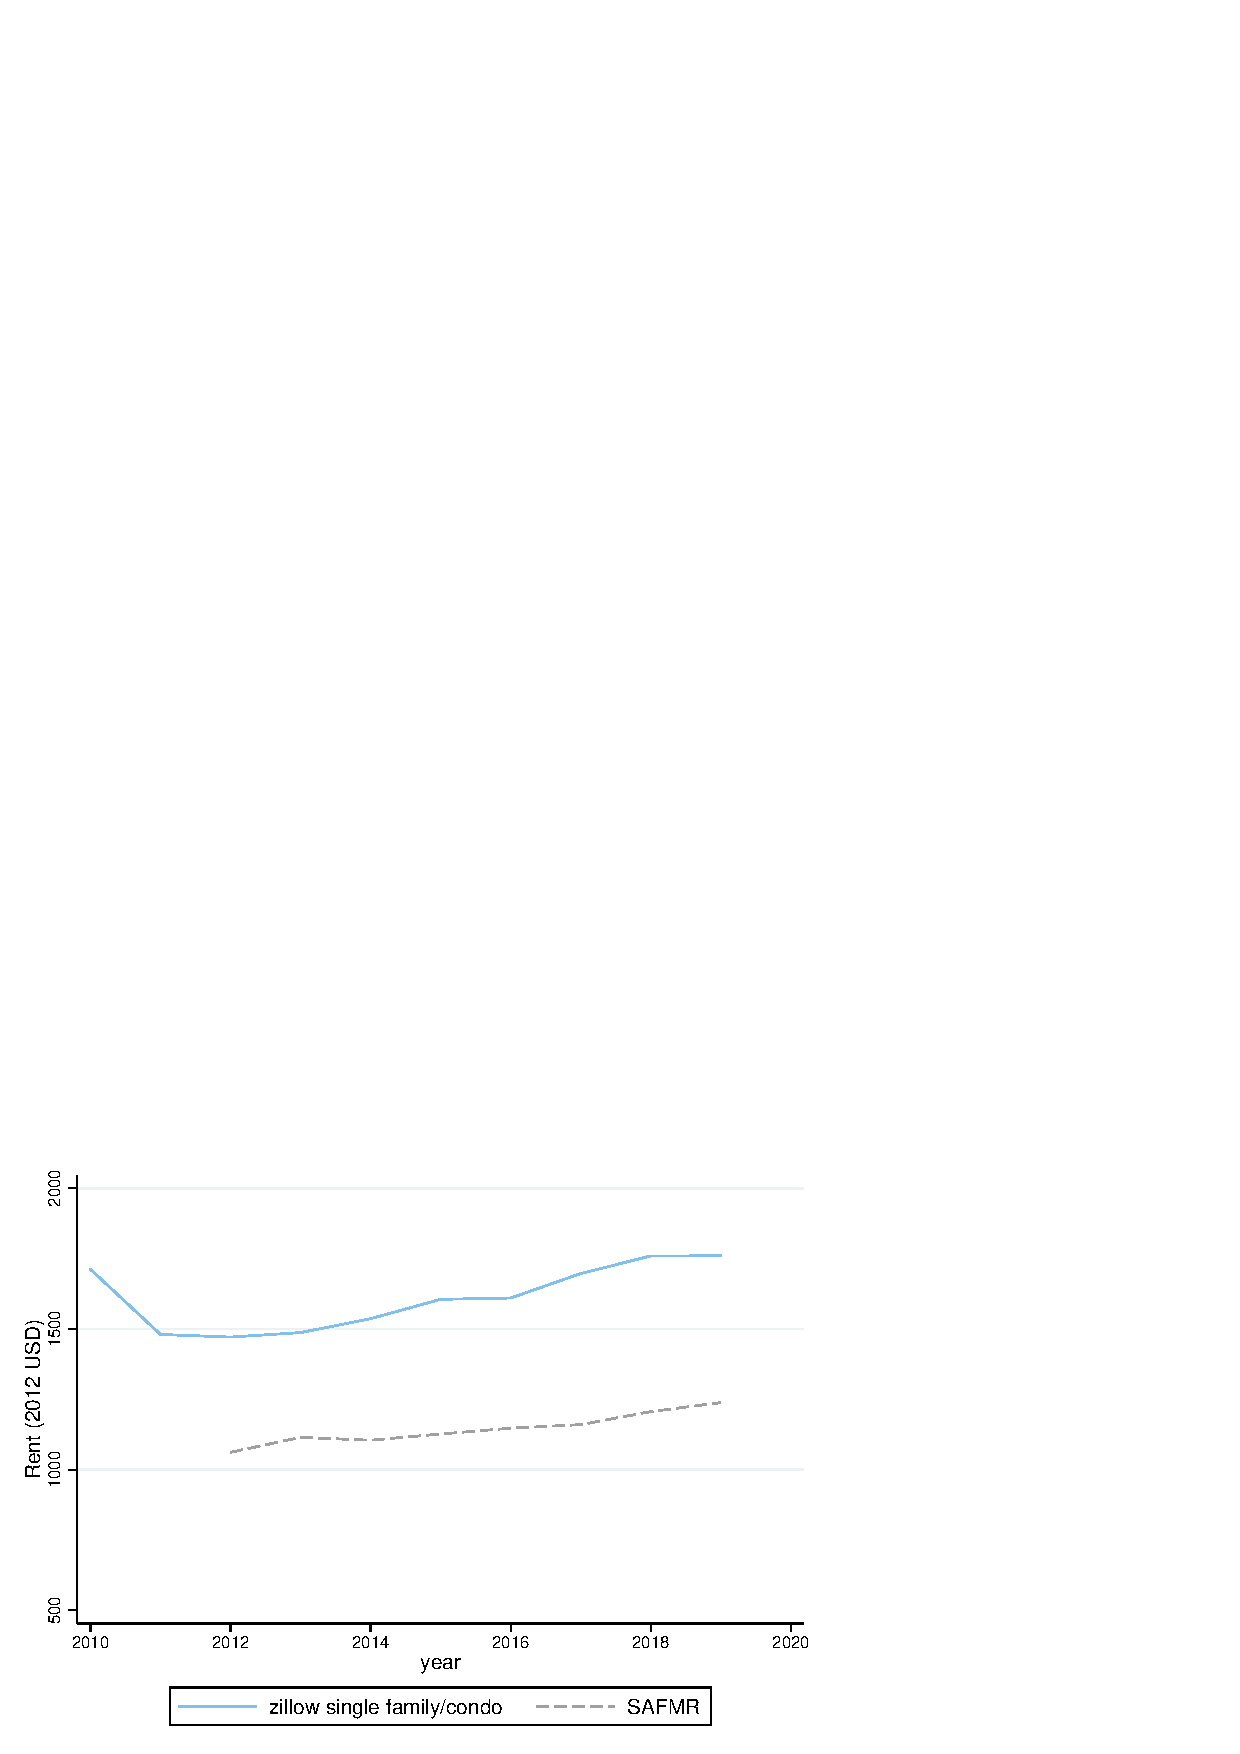
\includegraphics[width = 0.7\textwidth]{../analysis/zillow_benchmark/output/trend_zillow_safmrwgt_zipcode_avg.png}
    \begin{minipage}{0.95\textwidth} \footnotesize
    	\vspace{3mm}
    	\textit{Notes:} The figure plots the monthly rent annual national average for the main Zillow 
    	series used in the analysis (SFCC) and a weighted combination of SAFMR series with different 
    	number of bedrooms. Weights are based on the US share of single family, condos and cooperative 
    	houses with given number of bedrooms as recorded in the AHS.    
    \end{minipage}
\end{figure}

Third, we add socio-demographic information to each zipcode in our sample using the 2010 Census and 
the 5-years 2008-2012 ACS. The data is originally obtained at the Census tract level and mapped into 
USPS zipcodes using HUD crosswalks.\footnote{Crosswalks are obtained from
	 \url{https://www.huduser.gov/portal/datasets/usps_crosswalk.html}} 
We assign to each zipcode the following characteristics: number of inhabitants, the number of houses, 
the median income, the number of black inhabitants, the number of unemployed, and the number of 
college students. We use this information to classify zipcodes into, for example, high or low median 
income to then perform heterogeneity analysis. In addition, given that zipcodes can cross county 
borders, we use the census data and geographic codes to map each zipcode to a county by assigning it 
to the one with the highest share of houses from that zipcode. We also map each zipcode to a 
metropolitan statistical area or a rural town analogously. We use this information to assign the 
prevailing MW to each zipcode.

% Fourth, to proxy for the quality of amenities at each location, we construct zipcode-month level 
% measures from GPS location point-of-interest data by SafeGraph\parencite{safegraph}. We define several 
% amenity measures. For our first measure, we follow closely \textcite{couture2019income} and construct 
% an index for the quality of restaurants available at each zipcode-month. This index is defined as the 
% average of the propensity of high-income individuals to visit a restaurant in a given zipcode 
% controlling for their distance to the establishments. In order to classify a visitor as high-income we 
% use the census tract location of the visitor. Our second measure is the same as the first but for the 
% quality of the visitors of open public spaces in each zipcode-month. For our third measure, we use the 
% point-of-interest data to count the number of restaurants, coffee shops, bars, and gyms per inhabitant 
% of a zipcode-month. 

Fourth, to proxy for local economic activity we collect data from the Quarterly Census of Employment 
and Wages (QCEW) at the county-quarter and county-month level for each industry and level of 
government.\footnote{The QCEW covers the following industries: goods-producing; natural resources and 
	mining; construction; manufacturing; service-providing; trade, transportation and utilities; 
	information; financial activities; professional and business services; education and health 
	services; leisure and hospitality. The QCEW additionally provides employment data for federal, 
	state, and local government.} 
For each county-quarter-industry cell we observe the number of establishments and the average weekly 
wage. For each county-month-industry cell we additionally observe the number of employed people. We 
merge this data onto our zipcode-month panel based on county and quarterly date.

We add data from the \textit{Building Permit Survey} (BPS) at the county-month level to account for 
time-varying shocks in the housing market. The BPS provides building permit statistics on new 
privately-owned residential construction disaggregated by house type. Lacking information on condos 
and cooperative houses, we only add the number of new units and the permits valuation for single 
family houses to each zipcode-month observation based on the county and month they belong.

Finally, we use data from the 2017 Longitudinal Employer-Household Dynamics Origin-Destination 
Employment Statistics (LODES) to proxy for MW workers' residence and workplace location. The LODES 
data sets provide block-level information on jobs and are organized in 3 groups: residence area 
characteristics (RAC), with information about characteristics of jobs for various types of workers 
(e.g. number of jobs in different sectors, number of job for workers under 30 years old, etc.); 
workplace area characteristics (WAC) that provide the same information as RAC files but aggregated 
with respect to workplace location; and a origin-destination matrix mapping jobs from residence to 
workplace locations. We use RAC and WAC datasets to ``locate" workers likely to be MW by looking at 
the state-level distribution of such type of workers: we build, for each zipcode in the sample, the 
share (out of the state total) of workers under 30 years old earning less than $\$1251$ that either 
\textit{live} or \textit{work} there. 


\section{Empirical strategy and identification}\label{sec:empirical_strategy}
    %%%%%%%%%%%%%%%%%%%%%%%%%%%%%%%%%%%%%%%%%%%%%%%%%%%%%%%%%%%%%%%%%%%%%%%%%%%%%%%%%
%%%%%                         EMPIRICAL STRATEGY                             %%%%
%%%%%%%%%%%%%%%%%%%%%%%%%%%%%%%%%%%%%%%%%%%%%%%%%%%%%%%%%%%%%%%%%%%%%%%%%%%%%%%%%

In this section, we present the empirical strategy adopted to study the effect of MW on rents, and 
we discuss the assumptions needed for identification. We begin with a panel DiD model and we build 
on that following \textcite{meer2016effects}. This allows us to estimate the full dynamics of rents 
around MW changes under various identifying assumptions. Our dynamic specifications are distinct 
from the usual DiD and event-study ones \parencite{BorusyakJaravel2017, abraham2018} for two main 
reasons: first, our models allow for the use of variation coming from more than one MW change per 
geographic unit and from geographic units that never experience a MW change. This is desirable 
because we both avoid under-identification issues with the two-way fixed effects and because we 
use never-treated zipcodes as control units. Secondly, our specifications not only exploit the 
timing of a MW change for identification but also its intensity.
    
% Whereas this shows a statistically significant results, one may worry about pre-trends that 
% confound the effect. To account for this, in the dynamic model we add leads and lags of this 
% variable, which allows us to formally test the hypothesis of pre-trends.


%%%%%%%%%%%%%%%%%%%%%%%%%%%%%%%%%%%%%%%%%%%%%%%%%%%%%%%%%%%%%%%%%%%%%%%%%%%%%%%%%
\subsection{Baseline Specifications}
Consider the following panel difference-in-differences model relating rents and the minimum wage:

\begin{equation}\label{eq:did_lev}
    y_{it} = \alpha_i + \alpha_t + \gamma_i t + \beta \underline{w}_{it} + \epsilon_{it}
\end{equation}
    
where $y_{it}$ is the log rent per square foot for the Zillow SFCC series, $\underline{w}$ is the 
log of the minimum wage, $\alpha_i$ is a zipcode fixed effect, $\alpha_t$ is a time fixed effect, 
and $\gamma_i$ is a zipcode-specific linear trend.\footnote{We add a zipcode-specific linear trend 
	to allow for heterogeneity in the time path of zipcodes \parencite{angrist2008mostly}. In the 
	next section we additionally present results from models without zipcode-specific linear trends 
	as well as with zipcode-specific quadratic trends.} 
We then re-write \autoref{eq:did_lev} in first differences:
    
\begin{equation}\label{eq:did}
        \Delta y_{it} = \theta_t + \gamma_i + \beta \Delta \underline{w}_{it} + \Delta \epsilon_{it}
\end{equation}

We reference this model as \textit{static DiD}. We spell out the model in first differences because 
we believe that the unobserved shocks to rental prices are likely to be persistent over time. Both 
the first differences and the level models are consistent under similar assumption but the first 
difference model is more efficient if the shocks are serially correlated \parencite{wooldridge2010}.

Identification comes from assuming that within a zipcode the change in the level of the logarithm 
of the minimum wage is mean independent of the change in the unobserved shock $\Delta \epsilon_{it}$ 
conditional on the time fixed effects and the zipcode-specific linear trend. This implies that if 
the true effect is a one-time level change, then $\beta$ has a causal interpretation and it can be 
seen as the elasticity of the rent per square foot to the MW.
    
One potential concern with the static DiD model, is that, despite controlling for a zipcode-specific 
linear trend, preexisting time-paths of rents per square foot might be different in zipcodes that 
had a MW change relative to zipcodes that did not experienced a change. To assess if that is the 
case, one can extend the model to include leads of $\Delta \underline{w}_{it}$. In addition, one 
may be believe that the effect of MW changes on rents is not a one time discrete level jump but that 
it also affects the growth rate of rental prices. In such cases the estimated coefficient $\beta$ 
from \autoref{eq:did} might only have limited relevance in evaluating the policy of interest 
\parencite{callaway2019difference}. To allow for dynamics in the effects, we extend the model to 
also include lags of $\Delta \underline{w}_{it}$. The \textit{dynamic} model is

\begin{equation}\label{eq:leads_lags}
    \Delta y_{it} = \theta_t + \gamma_i + \sum_{r=-s}^{s}\beta_r \Delta \underline{w}_{i(t-r)} 
    				+ \Delta \epsilon_{it} \ ,
\end{equation}
where $s$ is the number of months of a symmetric window around the MW change. Note that this 
dynamic DiD model still allows for treatment and control groups to have different averages, even though it now requires a more stringent identification: 
\[E \left[ \Delta \epsilon_{it} \Delta \underline{w}_{it-r} \big| \theta_{t}, \gamma_{i} \right] = 0
	\ \ \forall r\in\{-s, ..., -1, 0, 1, ..., s\} \ . \] 
In this context, a violation of the identification assumption would require a change in MW to be 
systematically correlated with unobserved shocks to treated zipcode relative to untreated ones. 
Importantly, this model allows us to test whether $\beta_{-s} = \beta_{-s+1} = ... = \beta_{-1} = 0$, 
the well known pre-trends test, to establish whether there are significant rent responses preceding 
a change in MW. Under the assumption of no pre-trends, we can gain efficiency through estimating a 
model only with distributed lags as follows:

\begin{equation}\label{eq:lags}
        \Delta y_{it} = \theta_t + \gamma_i 
        		+ \sum_{r=0}^{s}\beta_r \Delta \underline{w}_{i(t-r)} 
        		+ \Delta \epsilon_{it} \ .
\end{equation}

This model allows us to estimate the dynamics of the logarithm of the rent per square foot around 
changes in the MW and we can recover the elasticity of rents to MW by summing $\beta_0$ to 
$\beta_{s}$. We present results from this model in the results section. In past settings using 
yearly data \parencite{tidemann2018mw,yamagishi2019minimum}, MW changes are so common in a given 
geographic area relative to the timespan of the data that it is very hard to credibly estimate the 
lags. Intuitively, this is the case because it is hard to distinguish which variation of the rental 
price is due to the current MW change or to a preceding one. In our estimates that concern is not 
justified, as given that we have month to month variation, we use short windows (5 months) in which 
there is no overlap in MW changes within a zipcode. The absence of pre-trends does not exhaust the 
potential threats to identification. Effects could still be driven by contemporaneous shocks 
systematically affecting both changes in rents and MW within a zipcode. To ease those concerns, we 
directly control for several county-level time-varying proxies of the health of the local labor and 
housing markets.\footnote{This amounts to adding a vector $\Delta X_{ct}$ on the right-hand side of 
	our models, where $c$ indexes counties, and we map zipcodes to a single county as explained in \autoref{sec:data}.} 
As mentioned in \autoref{sec:data}, part of the variation in the median rental price come from 
unobserved changes in the Zillow inventory for a given zipcode through time. This may pose a threat 
to identification...\textbf{TO FINISH}

Finally, in our appendix, we consider a dynamic panel specification to allow for full dynamics on 
the rental prices. The model then becomes

\begin{equation}\label{eq:ab_panel}
        \Delta y_{it} = \Delta y_{i(t-1)} + \theta_t + \gamma_i 
        		+ \sum_{r=0}^{s}\beta_r \Delta \underline{w}_{i(t-r)} 
        		+ \Delta \epsilon_{it} \ .
\end{equation}

However, by construction we now have that $\Delta y_{i(t-1)}$ is necessarily correlated with 
$\Delta \epsilon_{it}$. To address that, we take two separate approaches. First, we follow 
\textcite{arellano1991some} and, as it is customary in the literature, we instrument $\Delta 
y_{i(t-1)}$ with $\Delta y_{i(t-2)}$. Second, we follow \textcite{meer2016effects} and instrument 
$\Delta y_{i(t-1)}$ with an off-window lag of the change in the logarithm of the MW. In particular, 
as most of our models have a window $s=5$, we use as an instrument $\Delta \underline{w}_{i(t-6)}$. 
Intuitively, if there is an effect of MW changes to rents past MW changes should predict future 
rents and past MW changes should not be correlated with contemporaneous unobserved determinants 
of rents once we take into account the dynamic effect of MW on rents. 


%%%%%%%%%%%%%%%%%%%%%%%%%%%%%%%%%%%%%%%%%%%%%%%%%%%%%%%%%%%%%%%%%%%%%%%%%%%%%%%%%
\subsection{Heterogeneity by Zipcode Characteristics }

In order to allow for heterogeneous effects based on zipcode characteristics, and to make sure 
that our effects are driven by the zipcodes that are expected to have more MW earners, we extend the 
baseline panel difference-in-differences model defined in \autoref{eq:did} by interacting the local MW change with zipcode level characteristics. To minimize the possibility of any characteristic 
being endogenous to MW changes, we use use socio-demographic data that predate our panel. We take 
them from the 2010 Census and the 5-years 2008-2012 ACS. Then, the model we take to the data becomes

\begin{equation}\label{eq:diff_main_hetero} 
    \Delta y_{it} = \theta_t + \gamma_i 
    		+ \sum_{q = 1}^4 \beta_q \mathds{1}\{i \in q\} \Delta \underline{w}_{it} 
    		+ \Delta \epsilon_{it} \ ,
\end{equation}
where $q$ identifies quartiles of some zipcode level characteristic, and $\mathds{1}\{ \cdot \}$ is 
the indicator function. We report results for these models in \autoref{sec:heter}.

\section{Results}\label{sec:results}
    
In this section we outline the estimated impact of MW changes on rent and house prices. We first how show the estimated impact of MW changes - as captured by \autoref{eq:main_ziplevel} - [ADD INTRO RESULTS]. As introduced in \autoref{sec:empirical_strategy}, when restricting the sample to have only one event per unit, identification is only reached up to a linear trend. We then present results for the first different specification: the estimated \textit{average treatment effect} decreases to XX. 

\subsection{An event-study specification}\label{subsec:results/event-study}

In this subsection, we present estimation results using median rents as our dependent variable. We focus on the median rent per square foot for single family houses and condos as this is the most populated time series in the Zillow rent data. [ADD ZILLOW DATA TABLE TO APPENDIX?]. \\

\autoref{fig:event_level_sal_6} plots the relative event coefficients from \autoref{eq:main_ziplevel}, where the dependent variable is the zipcode-level median rent per square foot for single family houses, condos and coop housing. In this initial setting, an event is considered to be a MW change of at least $\$0.5$.  

\begin{figure}[h!]
    \centering
    \caption{Effects of a MW change of at least \$0.5 on single family rent per square foot (in dollars).}
    \scalebox{0.45}{
    \includegraphics{analysis/event_study/output/last_rentpsqft_sfcc_w6.png}
    }
    \subcaption*{\textit{Note}: The figure shows the estimated $\hat{\delta}_{t+k}$ coefficients from the baseline specification. For each zipcode, we  add the sum of unused events and county-level seasonality as additional controls ($X_{jt}$). Avearage MW change: $\$0.8$. Standard errors are clustered at the zipcode level.}
    \label{fig:event_level_sal_6}
\end{figure}

The figure shows a rather flat and not statistically significant pre-trend followed by a immediate impact of around ten cents on rent that remains stable in the following months. 
To better understand the magnitude of such effect, notice that in the present specification the average increase of the MW change is of $\$0.8$. This implies that, for a family of 2 minimum wagers woring 40 hours a week, this change represents an increase on the family income of approximately \$278.4.\footnote{The average month has 4.35 weeks.} Assuming that this representative single family consumes 1500 square feet of housing, the implied increase in monthly rent is of about \$150, which implies an on-impact pass-through from the MW change to rents of 53.9\%. If assuming that the treatment effect is given by averaging the 7 post event coefficient, then the implies pass-through is of about 64.4\%.

First note that, taken at face value this number seems slightly high given that the median US rent requires 28.4\% of the median incomes \parencite{bi}. However, a household with 2 full time minimum wagers making, for example, the federal minimum wage of \$7.25 will have an annual income of \$30276, only slightly above half of the median US household income of \$59430 in 2015, which suggests that the estimated pass-through is plausible. 

Second, we check the robustness of this result by changing the prominence of the MW changes. Specifically, In \autoref{appfig:event_level_robustness6} we use MW changes that comply to our sample criterion (explained in section 2) and are of at least \$0.25 and of at least \$0.75 instead of \$0.5. we show how, as we increase the size of the MW changes to be considered as an event, the estimated effect becomes more persistent in the periods following the change. 

To get a more precise estimate of the impact on low-income households, for each of the event definitions we bootstrap, clustering at the zipcode level, the whole computation of the pass-through (assuming that the relevant per square foot effect is the average of the post event coefficients). The results are presented in Table \ref{tab:bootstrap_table}, where the column (2) corresponds to Figure \ref{fig:event_level_sal_6}. Note that we compute the implied pass-through for 3 different housing size - 1000, 1500, and 2000 square feet - in order to cover a plausible range of values for the average rental of a single family with 2 MW earners. Finally, note that as in any event-study, we are using only the zipcodes that have at least one MW change in our period. The estimated pass-throughs are all significantly different from zero: looking at the first row of \autoref{tab:bootstrap_table} we can see how rents show an average increase of around $0.7$ percent across MW changes of various strength. 


\begin{table}[h!]
    \centering
    \caption{Bootstrap estimates of the main objects of interest}
    \resizebox{\textwidth}{!}{
    {
\def\sym#1{\ifmmode^{#1}\else\(^{#1}\)\fi}
\begin{tabular}{l*{3}{c}}
\hline\hline
            &\multicolumn{1}{c}{(1)}        &\multicolumn{1}{c}{(2)}        &\multicolumn{1}{c}{(3)}        \\
            &\multicolumn{1}{c}{MW changes of at least \$0.25}&\multicolumn{1}{c}{MW changes of at least \$0.5}&\multicolumn{1}{c}{MW changes of at least \$0.75}\\
\hline
Rent increase per square feet&                0.0216\sym{*}  &                 0.103\sym{***}&                0.0812\sym{***}\\
            &      [0.00126,0.0420]         &        [0.0434,0.162]         &        [0.0540,0.108]         \\
[1em]
Total rent increase (assuming 1000 square feet)&                 21.62\sym{*}  &                 102.6\sym{***}&                 81.19\sym{***}\\
            &         [1.264,41.97]         &         [43.40,161.8]         &         [53.96,108.4]         \\
[1em]
Total rent increase (assuming 1500 square feet)&                 32.43\sym{*}  &                 153.9\sym{***}&                 121.8\sym{***}\\
            &         [1.896,62.96]         &         [65.10,242.7]         &         [80.93,162.6]         \\
[1em]
Total rent increase (assuming 2000 square feet)&                 43.24\sym{*}  &                 205.2\sym{***}&                 162.4\sym{***}\\
            &         [2.528,83.94]         &         [86.80,323.7]         &         [107.9,216.9]         \\
[1em]
Increase in income of a household with 2 full time minimum wages&                 219.2\sym{***}&                 278.4\sym{***}&                 403.7\sym{***}\\
            &         [211.5,227.0]         &         [269.1,287.7]         &         [388.0,419.3]         \\
[1em]
Implied passthrough from MW to rents (assuming 1000 square feet)&                0.0986\sym{*}  &                 0.369\sym{***}&                 0.201\sym{***}\\
            &       [0.00523,0.192]         &         [0.156,0.581]         &         [0.133,0.269]         \\
[1em]
Implied passthrough from MW to rents (assuming 1500 square feet)&                 0.148\sym{*}  &                 0.553\sym{***}&                 0.302\sym{***}\\
            &       [0.00784,0.288]         &         [0.235,0.871]         &         [0.199,0.404]         \\
[1em]
Implied passthrough from MW to rents (assuming 2000 square feet)&                 0.197\sym{*}  &                 0.737\sym{***}&                 0.402\sym{***}\\
            &        [0.0105,0.384]         &         [0.313,1.161]         &         [0.266,0.539]         \\
\hline
Average MW change&                   .63         &                    .8         &                  1.16         \\
Number of zipcode-months&                 68713         &                 43716         &                 37837         \\
Number of Zipcodes&                   676         &                   440         &                   383         \\
Number of bootstrap repetitions&                   196         &                   199         &                   196         \\
\hline\hline
\end{tabular}
}

    }
    \subcaption*{\textit{Notes:} Square brackets display the 95\% bootstrapped confidence intervals. Income computations are done assuming 2 MW earners.}
    \label{tab:bootstrap_table}
\end{table}


Next, we highlight the importance of allowing for flexible year-month fixed effects that are specific to the county. We highlight how this is possible since we are focusing on zipcode level variation, and we clarify the importance of it by introducing a comparison with a simpler specification: Figure \ref{fig:event_level_2way} presents an event study plot analogous to Figure \ref{fig:event_level_sal_6} but using a simple two-way fixed effect specification, which in our case corresponds to zipcode and year-month fixed effects. In such case, all variation across time and zipcodes ends up being used to estimate the relative event coefficients. This however may cause the model to be misspecified if, for example, different states or counties or MSAs were follwing different time trends in rent prices, as it is probably the case. In particular, as within zipcode variation is not "de-trended", the relative event coefficients will be much harder to estimate as they will be confounded by such trend. \\

\begin{figure}[h!]
    \centering
    \caption{Two-way fixed effects specification. Effects of a MW change of at least \$0.5 on single family rent per square foot (in dollars). Standard errors are clustered at the zipcode level.}
    \label{fig:event_level_2way}
    \scalebox{0.45}{
    \includegraphics{analysis/event_study/output/two_way_last_medrentpricepsqft_sfcc6.png}
    }
    \subcaption*{\textit{Notes:} The figure shows the estimated $\hat{\delta}_{t+k}$ coefficients from two-way fixed effect specification at the zipcode-month level. Average MW change: $\$0.8$. Standard errors are clustered at the zipcode level.}
\end{figure}

In fact, we see that estimation of the relative coefficients is much noisier and lower in magnitude. The within variation R-squared (the percentage of the within variation in the data explained by the model) is of 0.0066. When allowing for county-specific time fixed effects and county-specific calendar months (to allow for flexible seasonality patterns) that were infeasible under the specifications in the previous literature we get the results shown in \ref{fig:event_level_sal_6} and a within variation R-squared of 0.0779, so that we are able to explain 12 times more the observed within zipcode variation. These results suggest that county-specific year-month and seasonal month variation are important determinants of monthly rent at the local level above and beyond what a two way fixed effects model could capture.

With the last result of this subsection, we show the importance of a granular analysis of MW changes by looking at the implications of aggregating our zipcode-month data at the county-quarter level\footnote{In order to use the data in the same unit as \textcite{tidemann2018mw,yamagishi2019minimum} we should have aggregated at the county-year. However, that involves dealing with overlap in the events for each county as we have many MW changes on subsequent years. Therefore, we aggregated the data at the county-quarter under the thought that we can only do better than at the county-year.}. Figure \ref{fig:event_level_county2way} plots the relative event coefficients for a two-way fixed effect specification at the county-quarter, for a window of 2 quarters around MW changes of at least \$0.5. Similar to \textcite{tidemann2018mw} results are very imprecise and point estimates are, if anything, negative. 

\begin{figure}[h!]
    \centering
    \caption{Two-way fixed effects county-quarter specification}
    \label{fig:event_level_county2way}
    \scalebox{0.45}{
    \includegraphics{analysis/event_study_county_quarter/output/last_rentpsqft_sfcc_w2.png}
    }
    \subcaption*{\textit{Notes:} The figure shows the effect of a MW change of at least \$0.5 on single family rent per square foot (in dollars). We plot the estimated coefficients from a two-way fixed effect specification at the county-quarter level. 
    Standard errors are clustered at the zipcode level.}
\end{figure}

\subsection{Panel difference-in-differences specifications}\label{subsec:results/first-differences}

\subsubsection{Baseline results}

In this section we present the results from models based on section 4.2. Table XXX shows results from the static model in first differences. Column 1 reports results only including two way fixed effects. Column 2 adds a zipcode-specific linear trend, and column 3 a zipcode specific quadratic trend. 

%Add Table fd_table.tex

In all cases the effects is significant, stable and a 10\% change in the MW implies around a 0.25\% increase in the rent per square foot. 

Next, in Table XXX we show results from a model with 5 leads and lags of the logarithm of the MW. Again, Column 1 reports results of a specification with two way fixed effects. Column 2 adds a zipcode-specific linear trend, and column 3 a zipcode specific quadratic trend. 

% Add table fd_dynamic_table.tex

We also report the p-value of a test of $\beta_{-5} = \beta_{-4} = ... = \beta_{-1} = 0$. In all 3 cases we comfortably fail to reject that all leads are equal to 0 at the 95\% level. This is evidence that the pre-existing time paths of rent per square foot in zipcodes where the MW changed is not significantly different that the one for zipcodes in which the change didn't happened on that same time period. Given this, we estimate a model in which we assume all the leads are 0, and we include 5 lags of the logarithm of the MW (we call this model the distributed lags model). The coefficients from this estimation, plus the ones from the specification including 5 leads and lags are plotted in Figure XXX along with the path of effects implied by the static and distributed lags model. 

%Add figure fd_models.png

We can see that there is no evidence of pretrends, and that the effects implied by the dynamic models are slightly larger than the ones implied by the static one.  


\subsubsection{Heterogeneity by income}

In order to explore whether the effects of MW on rents are mainly driven by "minimum wager" zipcodes we divide the set of zipcodes into median household income quintiles from the 2010 census and we run the following model:

\begin{equation}\label{eq:diff_main}
        \Delta \tilde{y}_{it} = \theta_t + \gamma_i + \sum_{q=1}^5 \beta_q \mathds{1}\{i\in q\} \Delta \tilde{MW}_{it}+ \Delta \epsilon_{it}
\end{equation}

Were $q$ indexes median household income quintiles, and $\mathds{1}\{i\in q\}$ is 1 if zipcode $i$ belongs to the $q$th quintile of median household income. 

The results are displayed in the following figure. As expected, zipcodes in the lower quintile have an effect that significant and much larger in magnitude the baseline effect on the full sample of zipcodes.   

\subsection{Assessing magnitude of the effects}\label{subsec:results/magnitude}




\section{Discussion}\label{sec:discussion}
	%%%%%%%%%%%%%%%%%%%%%%%%%%%%%%%%%%%%%%%%%%%%%%%%%%%%%%%%%%%%%%%%%%%%%%%%%%%%%%%%%
%%%%%                             DISCUSSION                                 %%%%
%%%%%%%%%%%%%%%%%%%%%%%%%%%%%%%%%%%%%%%%%%%%%%%%%%%%%%%%%%%%%%%%%%%%%%%%%%%%%%%%%

TO ADD

% Calculation (SH): 

% Consider a zipcode that increases the hourly minimum wage from \$ 10 to \$ 11, and assume a household composed of two minimum wagers who work full time and pay \$ 2,500 of monthly rent. This family will experience an increase in their yearly income of approximately 2 $\times$ \$ 1 $\times$ 50 weeks $\times$ 40 hours a week $ = $ \$ 4,000.\footnote{Assuming they do not work for 2 weeks in a year.} According to our estimates, they would pay an extra \$ 2,500 $\times$ 12 $\times$ 0.5 $ = $ \$ 150 of rent. 

\section{Conclusions}\label{sec:conclusion}
    \input{07conclusion}

 

%%%%%%%%%%%%%%%%%%%%%%%%%%%%%%%%%%%%%%%%%%%%%%%%%%%%%%%%%%%%%%%%%%%%%%%%%%%%%%%%%%
%%%%                                 TAIL                                     %%%%
%%%%%%%%%%%%%%%%%%%%%%%%%%%%%%%%%%%%%%%%%%%%%%%%%%%%%%%%%%%%%%%%%%%%%%%%%%%%%%%%%%

\clearpage
\nocite{*}
\printbibliography


\clearpage

\section*{\centering{Online Appendix}}
\vspace{5mm}

\appendix

\renewcommand\thetable{\thesection.\arabic{table}}    
\renewcommand\thefigure{\thesection.\arabic{figure}} 
\setcounter{table}{0}
\setcounter{figure}{0}

\section{Appendix Tables}
	%%%%%%%%%%%%%%%%%%%%%%%%%%%%%%%%%%%%%%%%%%%%%%%%%%%%%%%%%%%%%%%%%%%%%%%%%%%%%%%%%
%%%%%                           APPENDIX TABLES                              %%%%
%%%%%%%%%%%%%%%%%%%%%%%%%%%%%%%%%%%%%%%%%%%%%%%%%%%%%%%%%%%%%%%%%%%%%%%%%%%%%%%%%

\begin{table}[h!]
	\caption{Dynamic DiD: cumulative effect over 6 months}
	\label{tab:dynamic_cumulative}
	\centering
	\resizebox{0.7\textwidth}{!}{
		\vspace{0pt}    
		{
\def\sym#1{\ifmmode^{#1}\else\(^{#1}\)\fi}
\begin{tabular}{l*{5}{c}}
\hline\hline
          &\multicolumn{1}{c}{(1)}         &\multicolumn{1}{c}{(2)}         &\multicolumn{1}{c}{(3)}         &\multicolumn{1}{c}{(4)}         &\multicolumn{1}{c}{(5)}         \\
\hline
Sum of MW effects&   0.0566         &   0.0554         &   0.0562         &   0.0563         &   0.0556         \\
          & (0.0347)         & (0.0345)         & (0.0343)         & (0.0343)         & (0.0342)         \\
\hline
Wage controls&       No         &      Yes         &      Yes         &       No         &      Yes         \\
Employment controls&       No         &       No         &       No         &       No         &      Yes         \\
Establishment-count controls&       No         &       No         &       No         &      Yes         &      Yes         \\
Observations&  106,446         &  104,360         &  104,360         &  106,160         &  104,360         \\
\hline\hline
\end{tabular}
}

	}
	\begin{minipage}{.95\textwidth} \footnotesize
		\vspace{3mm} 
		\textit{Notes}: The table shows estimates for the cumulative impact of MW (log) changes 
		on (log) rents changes over 6 months. Coefficients are obtained by taking the sum of 
		$\hat{\beta}_{r}$, estimated via \autoref{eq:lags}: $\sum\limits_{r=0}^{5} \hat{\beta}_{r}$. 
		Standard errors clustered at the state level. *** $p < 0.01$, ** $p < 0.05$, * $p < 0.1$.   
	\end{minipage}
\end{table}

\clearpage
\begin{landscape}
	\begin{table}[h!]
	    \caption{Results from different dynamic models}
	    \label{tab:horse_race_main}
	    \centering
	    \resizebox{1.2\textwidth}{!}{
		    \vspace{0pt}    
		    {
\def\sym#1{\ifmmode^{#1}\else\(^{#1}\)\fi}
\begin{tabular}{l*{5}{c}}
\hline\hline
          &\multicolumn{1}{c}{(1)}&\multicolumn{1}{c}{(2)}&\multicolumn{1}{c}{(3)}&\multicolumn{1}{c}{(4)}&\multicolumn{1}{c}{(5)}\\
          &\multicolumn{1}{c}{DiD}&\multicolumn{1}{c}{Distributed leads and lags}&\multicolumn{1}{c}{Distributed Lags}&\multicolumn{1}{c}{AB distributed leads and lags}&\multicolumn{1}{c}{AB distributed lags}\\
\hline
\Delta ln(MW)\_{t-3}&                  & 0.000493         &                  & 0.000164         &                  \\
          &                  &(0.00833)         &                  &(0.00889)         &                  \\
[1em]
\Delta ln(MW)\_{t-2}&                  &  0.00520         &                  &  0.00527         &                  \\
          &                  & (0.0122)         &                  & (0.0112)         &                  \\
[1em]
\Delta ln(MW)\_{t-1}&                  & -0.00115         &                  & -0.00262         &                  \\
          &                  & (0.0130)         &                  & (0.0107)         &                  \\
[1em]
\Delta ln(MW)\_{t}&   0.0256\sym{**} &   0.0267\sym{**} &   0.0261\sym{**} &   0.0265\sym{**} &   0.0261\sym{**} \\
          & (0.0121)         & (0.0123)         & (0.0126)         & (0.0107)         & (0.0109)         \\
[1em]
\Delta ln(MW)\_{t+1}&                  &   0.0161\sym{*}  &   0.0158\sym{*}  &   0.0225\sym{**} &   0.0223\sym{**} \\
          &                  &(0.00833)         &(0.00812)         &(0.00943)         &(0.00938)         \\
[1em]
\Delta ln(MW)\_{t+2}&                  & -0.00758         & -0.00714         & -0.00381         & -0.00331         \\
          &                  & (0.0126)         & (0.0128)         & (0.0132)         & (0.0134)         \\
[1em]
\Delta ln(MW)\_{t+3}&                  &  0.00280         &  0.00342         &  0.00117         &  0.00195         \\
          &                  &(0.00832)         &(0.00819)         &(0.00983)         &(0.00978)         \\
[1em]
\Delta ln(y)\_{t-1}&                  &                  &                  &   -0.241\sym{***}&   -0.239\sym{***}\\
          &                  &                  &                  &(0.00633)         &(0.00618)         \\
\hline
R-squared &    0.024         &    0.024         &    0.024         &    0.081         &    0.080         \\
Observations&   112232         &   108780         &   112209         &   107654         &   111083         \\
\hline\hline
\end{tabular}
}

	    }
	    \begin{minipage}{1.15\textwidth} \footnotesize
			\vspace{3mm} 
			\textit{Notes}: The table presents baseline estimates obtained from \autoref{eq:did}, 
			(\ref{eq:leads_lags}), and (\ref{eq:lags}) in columns (1), (2), and (3) respectively. 
			Column (4) allows for rental price dynamics by adding the lagged change in (log) rents, 
			$\Delta y_{i(t-1)}$, and it is estimated instrumenting it with a deeper lag $\Delta 
			y_{i(t-2)}$ \parencite{arellano1991some}. Similarly, column (5) solves for 
			\autoref{eq:ab_panel} where only lags of MW changes are allowed. Finally, columns (6) and 
			(7) instrument $\Delta y_{i(t-1)}$ with an off-window lag of the MW (log) change, $\Delta 
			\title{MW}_{i(t-6)}$ for the leads and lags, and lags only versions of the model. All 
			specifications additionally control for a zipcode-level linear trend. Standard errors 
			clustered at the state level. *** $p < 0.01$, ** $p < 0.05$, * $p < 0.1$.   
		\end{minipage}
	\end{table}
\end{landscape}

\clearpage
\begin{table}[h!]
    \caption{Comparison between unbalanced and baseline panel model estimation}
    \label{tab:comparison_unbal_base}
    \centering
     \resizebox{\textwidth}{!}{
    \vspace{0pt}    
    {
\def\sym#1{\ifmmode^{#1}\else\(^{#1}\)\fi}
\begin{tabular}{l*{6}{c}}
\hline\hline
          &\multicolumn{3}{c}{Unbalanced Panel}                    &\multicolumn{3}{c}{Baseline Panel}                      \\\cmidrule(lr){2-4}\cmidrule(lr){5-7}
          &\multicolumn{1}{c}{(1)}&\multicolumn{1}{c}{(2)}&\multicolumn{1}{c}{(3)}&\multicolumn{1}{c}{(4)}&\multicolumn{1}{c}{(5)}&\multicolumn{1}{c}{(6)}\\
          &\multicolumn{1}{c}{DiD}&\multicolumn{1}{c}{\shortstack{Distributed \\ leads and lags}}&\multicolumn{1}{c}{\shortstack{Distributed \\ Lags}}&\multicolumn{1}{c}{DiD}&\multicolumn{1}{c}{\shortstack{Distributed \\ leads and lags}}&\multicolumn{1}{c}{\shortstack{Distributed \\ Lags}}\\
\hline
$\Delta \ln(MW)_{t-5}$&                  &  -0.0115         &                  &                  &  -0.0153         &                  \\
          &                  &(0.00810)         &                  &                  &(0.00915)         &                  \\
[1em]
$\Delta \ln(MW)_{t-4}$&                  & -0.00812         &                  &                  & -0.00306         &                  \\
          &                  &(0.00792)         &                  &                  & (0.0110)         &                  \\
[1em]
$\Delta \ln(MW)_{t-3}$&                  & -0.00171         &                  &                  & 0.000380         &                  \\
          &                  &(0.00864)         &                  &                  &(0.00829)         &                  \\
[1em]
$\Delta \ln(MW)_{t-2}$&                  & -0.00233         &                  &                  &  0.00531         &                  \\
          &                  &(0.00743)         &                  &                  & (0.0121)         &                  \\
[1em]
$\Delta \ln(MW)_{t-1}$&                  &  0.00552         &                  &                  &-0.000798         &                  \\
          &                  &(0.00823)         &                  &                  & (0.0126)         &                  \\
[1em]
$\Delta \ln(MW)_{t}$&   0.0220\sym{*}  &   0.0218\sym{*}  &   0.0229\sym{*}  &   0.0257\sym{**} &   0.0265\sym{**} &   0.0268\sym{**} \\
          & (0.0111)         & (0.0117)         & (0.0115)         & (0.0120)         & (0.0119)         & (0.0126)         \\
[1em]
$\Delta \ln(MW)_{t+1}$&                  &  0.00473         &  0.00788         &                  &   0.0128\sym{*}  &   0.0162\sym{*}  \\
          &                  &(0.00574)         &(0.00586)         &                  &(0.00739)         &(0.00816)         \\
[1em]
$\Delta \ln(MW)_{t+2}$&                  &  0.00405         &  0.00558         &                  & -0.00785         & -0.00623         \\
          &                  &(0.00915)         &(0.00772)         &                  & (0.0135)         & (0.0128)         \\
[1em]
$\Delta \ln(MW)_{t+3}$&                  &  0.00347         &  0.00638         &                  &  0.00277         &  0.00359         \\
          &                  &(0.00632)         &(0.00636)         &                  &(0.00751)         &(0.00830)         \\
[1em]
$\Delta \ln(MW)_{t+4}$&                  &  0.00515         &  0.00505         &                  &  0.00994         &   0.0108         \\
          &                  &(0.00688)         &(0.00684)         &                  &(0.00695)         &(0.00704)         \\
[1em]
$\Delta \ln(MW)_{t+5}$&                  & 0.000767         & -0.00261         &                  &  0.00778         &  0.00641         \\
          &                  &(0.00774)         &(0.00800)         &                  &(0.00735)         &(0.00691)         \\
\hline
Observations&   194295         &   177659         &   194209         &   112232         &   106446         &   112161         \\
\hline\hline
\end{tabular}
}

    }
    \begin{minipage}{.95\textwidth} \footnotesize
		\vspace{3mm} 
		\textit{Notes}: The table compares estimates from our main specifications (\textit{static DiD}, 
		\textit{distributed leads and lags DiD}, and \textit{distributed lags DiD}) obtained using the 
		baseline sample with estimates obtained using the unbalanced, full sample of zipcodes. Columns 
		(1), (2), and (3) show results from from \autoref{eq:did}, (\ref{eq:leads_lags}), and (\ref{eq:lags}) 
		respectively, using the unbalanced sample. All three columns additionally control for ``cohort 
		$\times$ period" FE to account for differences in the each zipcodes time series. Columns (4), (5), 
		and (6) replicates our main results obtained with the baseline sample and presented in 
		\autoref{tab: did_main}, column (2), \autoref{tab: dynamic_lags_leads_main}, column (2) and 
		\autoref{tab:horse_race_main}. All specifications control for zipcode-level linear trends. 
		Standard errors clustered at the state level. *** $p < 0.01$, ** $p < 0.05$, * $p < 0.1$.  
	\end{minipage}
\end{table}

\clearpage
\begin{table}[h!]
    \caption{Comparison between baseline and re-weighted panel model estimation}
    \label{tab:comparison_wgt_base}
    \centering
    \resizebox{\textwidth}{!}{
	    \vspace{0pt}    
	    {
\def\sym#1{\ifmmode^{#1}\else\(^{#1}\)\fi}
\begin{tabular}{l*{6}{c}}
\hline\hline
          &\multicolumn{3}{c}{Reweighted Panel}                    &\multicolumn{3}{c}{Baseline Panel}                      \\\cmidrule(lr){2-4}\cmidrule(lr){5-7}
          &\multicolumn{1}{c}{(1)}&\multicolumn{1}{c}{(2)}&\multicolumn{1}{c}{(3)}&\multicolumn{1}{c}{(4)}&\multicolumn{1}{c}{(5)}&\multicolumn{1}{c}{(6)}\\
          &\multicolumn{1}{c}{DiD}&\multicolumn{1}{c}{\shortstack{Distributed \\ leads and lags}}&\multicolumn{1}{c}{\shortstack{Distributed \\ Lags}}&\multicolumn{1}{c}{DiD}&\multicolumn{1}{c}{\shortstack{Distributed \\ leads and lags}}&\multicolumn{1}{c}{\shortstack{Distributed \\ Lags}}\\
\hline
$\Delta \ln(MW)_{t-5}$&                  & -0.00832         &                  &                  &  -0.0153         &                  \\
          &                  &(0.00687)         &                  &                  &(0.00915)         &                  \\
[1em]
$\Delta \ln(MW)_{t-4}$&                  &  0.00566         &                  &                  & -0.00306         &                  \\
          &                  &(0.00726)         &                  &                  & (0.0110)         &                  \\
[1em]
$\Delta \ln(MW)_{t-3}$&                  &  0.00821         &                  &                  & 0.000380         &                  \\
          &                  &(0.00905)         &                  &                  &(0.00829)         &                  \\
[1em]
$\Delta \ln(MW)_{t-2}$&                  &-0.000403         &                  &                  &  0.00531         &                  \\
          &                  & (0.0115)         &                  &                  & (0.0121)         &                  \\
[1em]
$\Delta \ln(MW)_{t-1}$&                  & -0.00860         &                  &                  &-0.000798         &                  \\
          &                  & (0.0116)         &                  &                  & (0.0126)         &                  \\
[1em]
$\Delta \ln(MW)_{t}$&   0.0365\sym{***}&   0.0369\sym{***}&   0.0372\sym{***}&   0.0257\sym{**} &   0.0265\sym{**} &   0.0268\sym{**} \\
          & (0.0124)         & (0.0127)         & (0.0132)         & (0.0120)         & (0.0119)         & (0.0126)         \\
[1em]
$\Delta \ln(MW)_{t+1}$&                  &  0.00782         &  0.00942         &                  &   0.0128\sym{*}  &   0.0162\sym{*}  \\
          &                  &(0.00706)         &(0.00730)         &                  &(0.00739)         &(0.00816)         \\
[1em]
$\Delta \ln(MW)_{t+2}$&                  & -0.00822         & -0.00694         &                  & -0.00785         & -0.00623         \\
          &                  & (0.0167)         & (0.0160)         &                  & (0.0135)         & (0.0128)         \\
[1em]
$\Delta \ln(MW)_{t+3}$&                  &  0.00560         &  0.00516         &                  &  0.00277         &  0.00359         \\
          &                  &(0.00600)         &(0.00693)         &                  &(0.00751)         &(0.00830)         \\
[1em]
$\Delta \ln(MW)_{t+4}$&                  &   0.0100         &   0.0103         &                  &  0.00994         &   0.0108         \\
          &                  &(0.00939)         &(0.00935)         &                  &(0.00695)         &(0.00704)         \\
[1em]
$\Delta \ln(MW)_{t+5}$&                  &  0.00798         &  0.00781         &                  &  0.00778         &  0.00641         \\
          &                  &(0.00808)         &(0.00870)         &                  &(0.00735)         &(0.00691)         \\
\hline
Observations&  112,232         &  106,446         &  112,161         &  112,232         &  106,446         &  112,161         \\
\hline\hline
\end{tabular}
}

    }
    \begin{minipage}{.95\textwidth} \footnotesize
		\vspace{3mm} 
		\textit{Notes}: The table compares estimates from our main specifications (\textit{static 
		DiD}, \textit{distributed leads and lags DiD}, and \textit{distributed lags DiD}) obtained 
		using the baseline sample with estimates obtained using the reweighted sample (see 
		\autoref{sec:sample_rest} for more details on how the weights are built). Columns (1), (2), 
		and (3) show results from from \autoref{eq:did}, (\ref{eq:leads_lags}), and (\ref{eq:lags}) 
		respectively, using the unbalanced sample. All three columns additionally control for 
		``cohort $\times$ period" FE to account for differences in the each zipcodes time series. 
		Columns (4), (5), and (6) replicates our main results obtained with the baseline sample 
		and presented in \autoref{tab: did_main}, column (2), \autoref{tab: dynamic_lags_leads_main}, 
		column (2) and \autoref{tab:horse_race_main}. All specifications control for zipcode-level 
		linear trends. Standard errors clustered at the state level. *** $p < 0.01$, ** $p < 0.05$, 
		* $p < 0.1$.
	\end{minipage}
\end{table}

\clearpage
\section{Appendix Figures}
	%%%%%%%%%%%%%%%%%%%%%%%%%%%%%%%%%%%%%%%%%%%%%%%%%%%%%%%%%%%%%%%%%%%%%%%%%%%%%%%%%
%%%%%                          APPENDIX FIGURES                              %%%%
%%%%%%%%%%%%%%%%%%%%%%%%%%%%%%%%%%%%%%%%%%%%%%%%%%%%%%%%%%%%%%%%%%%%%%%%%%%%%%%%%

\begin{figure}[!h]
    \caption{Dynamic DiD model comparison - local shocks}
    \label{fig:}
    \centering
    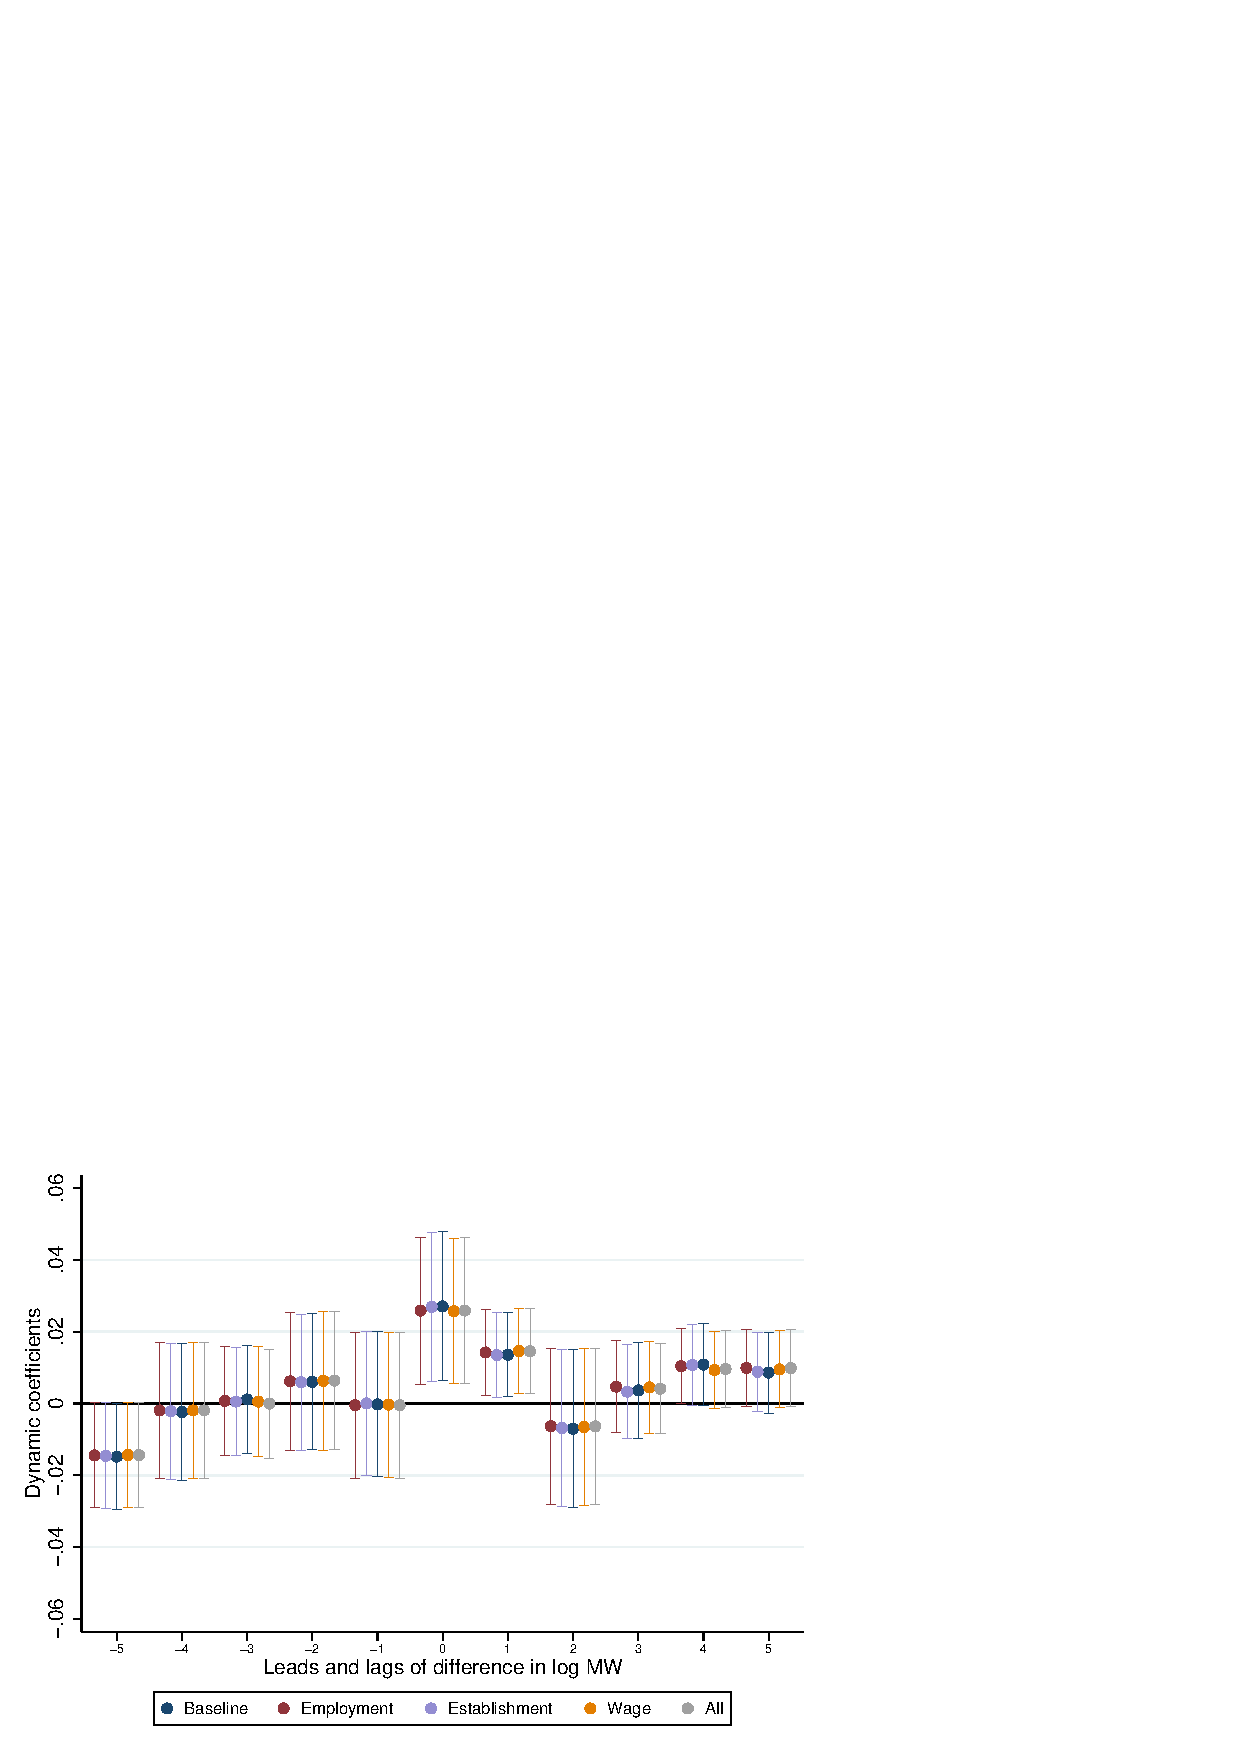
\includegraphics[width = 0.7\textwidth]{../../analysis/first_differences/output/fd_models_control.png}
    \begin{minipage}{.95\textwidth} \footnotesize
		\vspace{2mm} 
		\textit{Notes}: The figure show estimates for $\hat{\beta}_{r}$ obtained from 
		\autoref{eq:leads_lags} when progressively adding time-varying controls for local shocks. 
		The \textit{baseline} series plots coefficients taken from 
		\autoref{tab:dynamic_leads_lags_econshock}, column (1). The \textit{employment}, 
		\textit{establishment}, \textit{wage}, and \textit{building} series plot coefficients 
		from \autoref{tab:dynamic_leads_lags_econshock}, columns (2) to (5) respectively. 90 
		percent confidence intervals reported.  
	\end{minipage}
\end{figure}



\end{document}